%%
%  ******************************************************************************
%  * #file    Szablon_raportu_EN_Latex.tex
%  * #author  Adrian Wójcik   adrian.wojcik(at)put.poznan.pl
%  *          
%  * #commit  Patryk Kościk   koscikpatryk(at)gmail.com
%  *          Modified the template for Projekt przejsciowy purposes          
%  *          
%  * #version 1.0
%  * #date    09-Mar-2022
%  * #brief   PROJPRZEJ
%  *
%  ******************************************************************************
%%  
\documentclass[11pt, a4paper]{article}

\usepackage{SM_template}

% Wypełnijcie te dyrektywy zgodnie z waszym tematem
% \lab      -> NAZWA CZUJNIKA, np.: 'DHT22'
% \comment  -> Króciutki opis co to, np.: 'Cyfrowy budżetowy czujnik temperatury'
%

\lab{Moduł KY-018}
\comment{Analogowy czujnik natężenia światła}
\author{Dawid Wasung}
\addbibresource{bib/KY-018.bib}

% Absolutny zakaz dotykania tego tutaj bo jak dotkiecie to coś jebnie
\university{Politechnika Poznańska}
\faculty{Wydział Automatyki, Robotyki i Elektrotechniki}
\institute{Instytut Robotyki i Inteligencji Maszynowej}
\department{Zakład Sterowania i Elektroniki Przemysłowej}

\nocite{*}


%%
%
% Początek dokumentu
%
%%
\begin{document}

%% Strona tytułowa %%
\mainpage{{KY-018/foto}}
\newpage

\section*{Opis elementu} \addcontentsline{toc}{section}{Wstęp}
Fotorezystor jest elementem półprzewodnikowym, którego rezystancja ulega zmianie pod wpływem padającego na niego promieniowania elektromagnetycznego; przykładowo promieniowania widzialnego lub podczerwieni. Rezystancja elementu zależy od natężenia oświetlenia fotorezystora, jego rezystancja w ciemności jest bardzo duża i może osiągnąć wartość rzędu megaomów, przy silnym oświetleniu może zmaleć do kilku omów. Fotorezystor posiada dwa wyprowadzenia oraz charakterystyczną powierzchnię światłoczułą, na której znaleźć można grzebieniowe elektrody podłączone do 2 wyprowadzeń. Fotorezystory są wykonywane z półprzewodnika (np. krzemu lub siarczku ołowiu), który naniesiony jest na szklane podłoże. Światło padające na czujnik generuje nośniki ładunku elektrycznego, co ułatwia przepływ prądu. 
\vspace{0.5cm}
\begin{figure}[h!]
\centering
\begin{subfigure}{.5\textwidth}
  \centering
  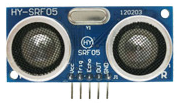
\includegraphics[width=.74\linewidth]{fig/KY-018/zdj_modułu/fig2.png}
  \caption{Moduł KY-018 \cite{ArduinoModules:grab}}
  \label{fig:sub1}
\end{subfigure}%
\begin{subfigure}{.5\textwidth}
  \centering
  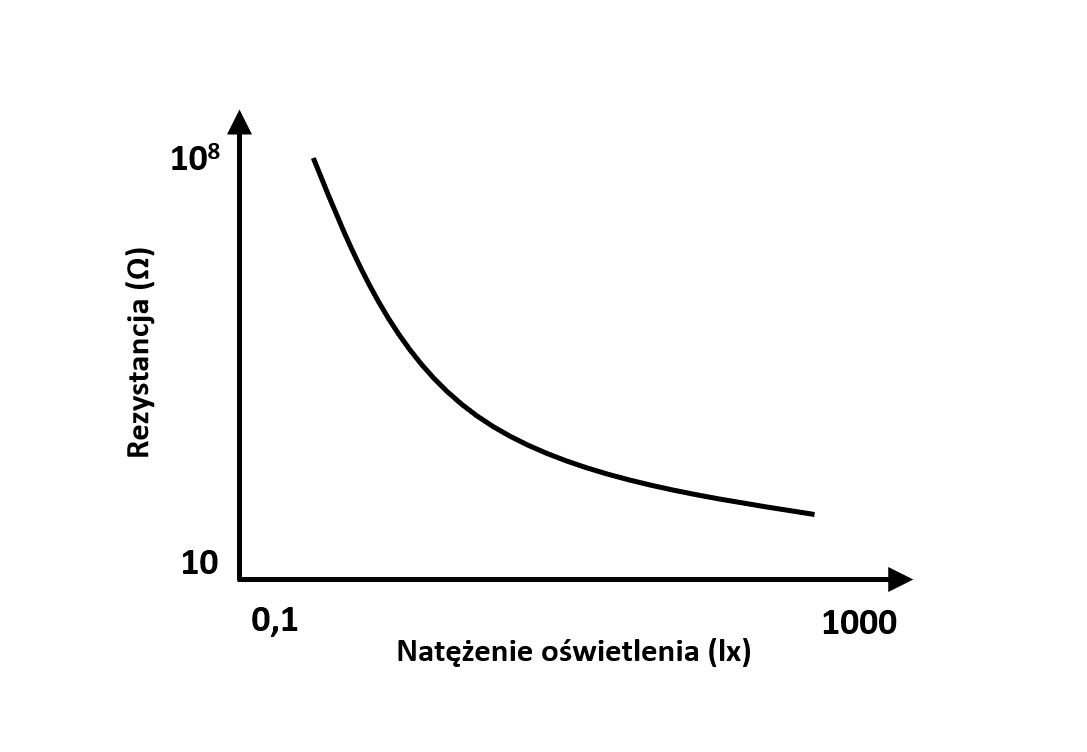
\includegraphics[width=1.05\linewidth]{fig/KY-018/zasada_dzialania/Charakterystyka.png}
  \caption{Zależność rezystancji od natężenia światła \cite{Foto:Wiki}}
  \label{fig:sub2}
\end{subfigure}
\caption{Poglądowe rysunki modułu oraz fotorezystora}
\label{fig:test}
\end{figure}
\newline
Czujnik KY-018 składa się z fotorezystora, wbudowanego rezystora 10k $\Omega$ oraz trzech pinów męskich - odpowiednio dla zasilania, GND oraz sygnału. 

\begin{figure}[h!]
\centering
\begin{subfigure}{.5\textwidth}
  \centering
  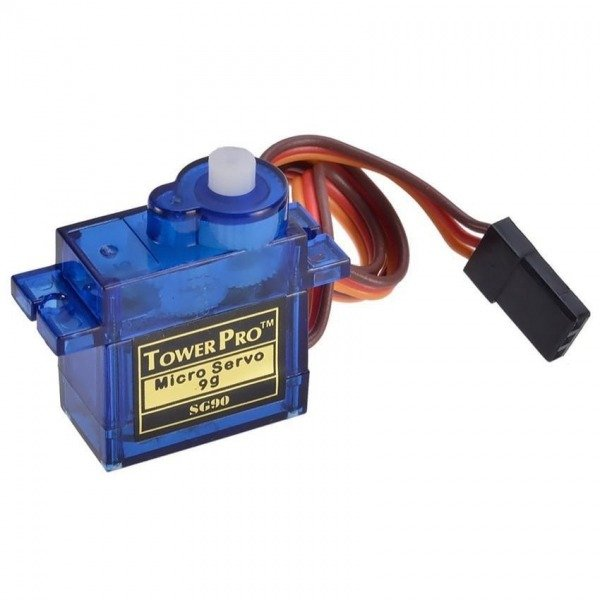
\includegraphics[width=.4\linewidth]{fig/KY-018/zdj_modułu/fig1.png}
  \caption{Moduł KY-018 \cite{ArduinoModules:Switch}}
  \label{fig:sub1}
\end{subfigure}%
\begin{subfigure}{.5\textwidth}
  \centering
  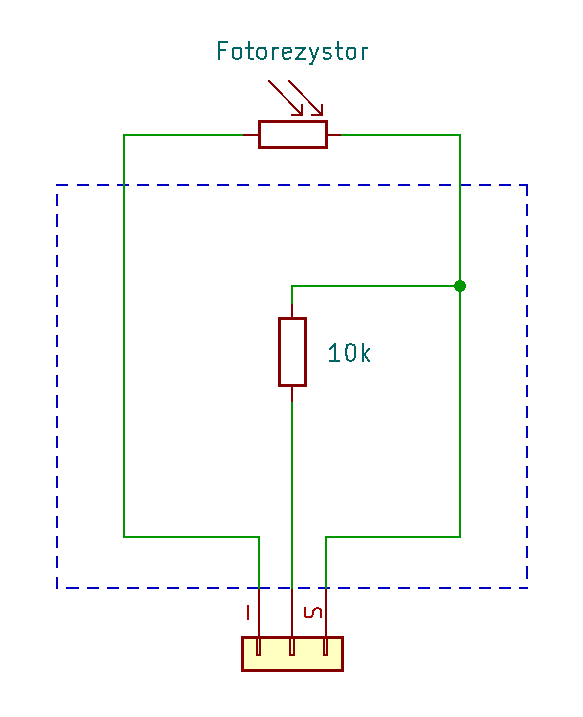
\includegraphics[width=0.6\linewidth]{fig/KY-018/zasada_dzialania/schemacik.png}
  \caption{Schemat modułu}
  \label{fig:sub2}
\end{subfigure}
\caption{Poglądowe rysunki modułu oraz fotorezystora}
\label{fig:test}
\end{figure}

\newpage
\section*{Użycie czujnika}
Zmianę rezystancji w zależności od natężenia światła określa charakterystyka rezystancyjno-oświetleniowa:
$$R_{E}=R_{0}(\frac{E_{0}}{E})^g$$
gdzie:
\begin{itemize}
    \item $R_{0}$ - rezystancja fotorezystora przy danym natężeniu światła $E_0$
    \item $E$ - natężenie oświetlenia
    \item $g$ - współczynnik zależny od rodzaju materiału półprzewodnikowego
\end{itemize}
Poniżej przedstawiono zmianę rezystancji modułu w zależności od zakrycia powierzchni światłoczułej (ograniczenie dostępu do światła).
\begin{figure}[h!]
\centering
\begin{subfigure}{.5\textwidth}
  \centering
  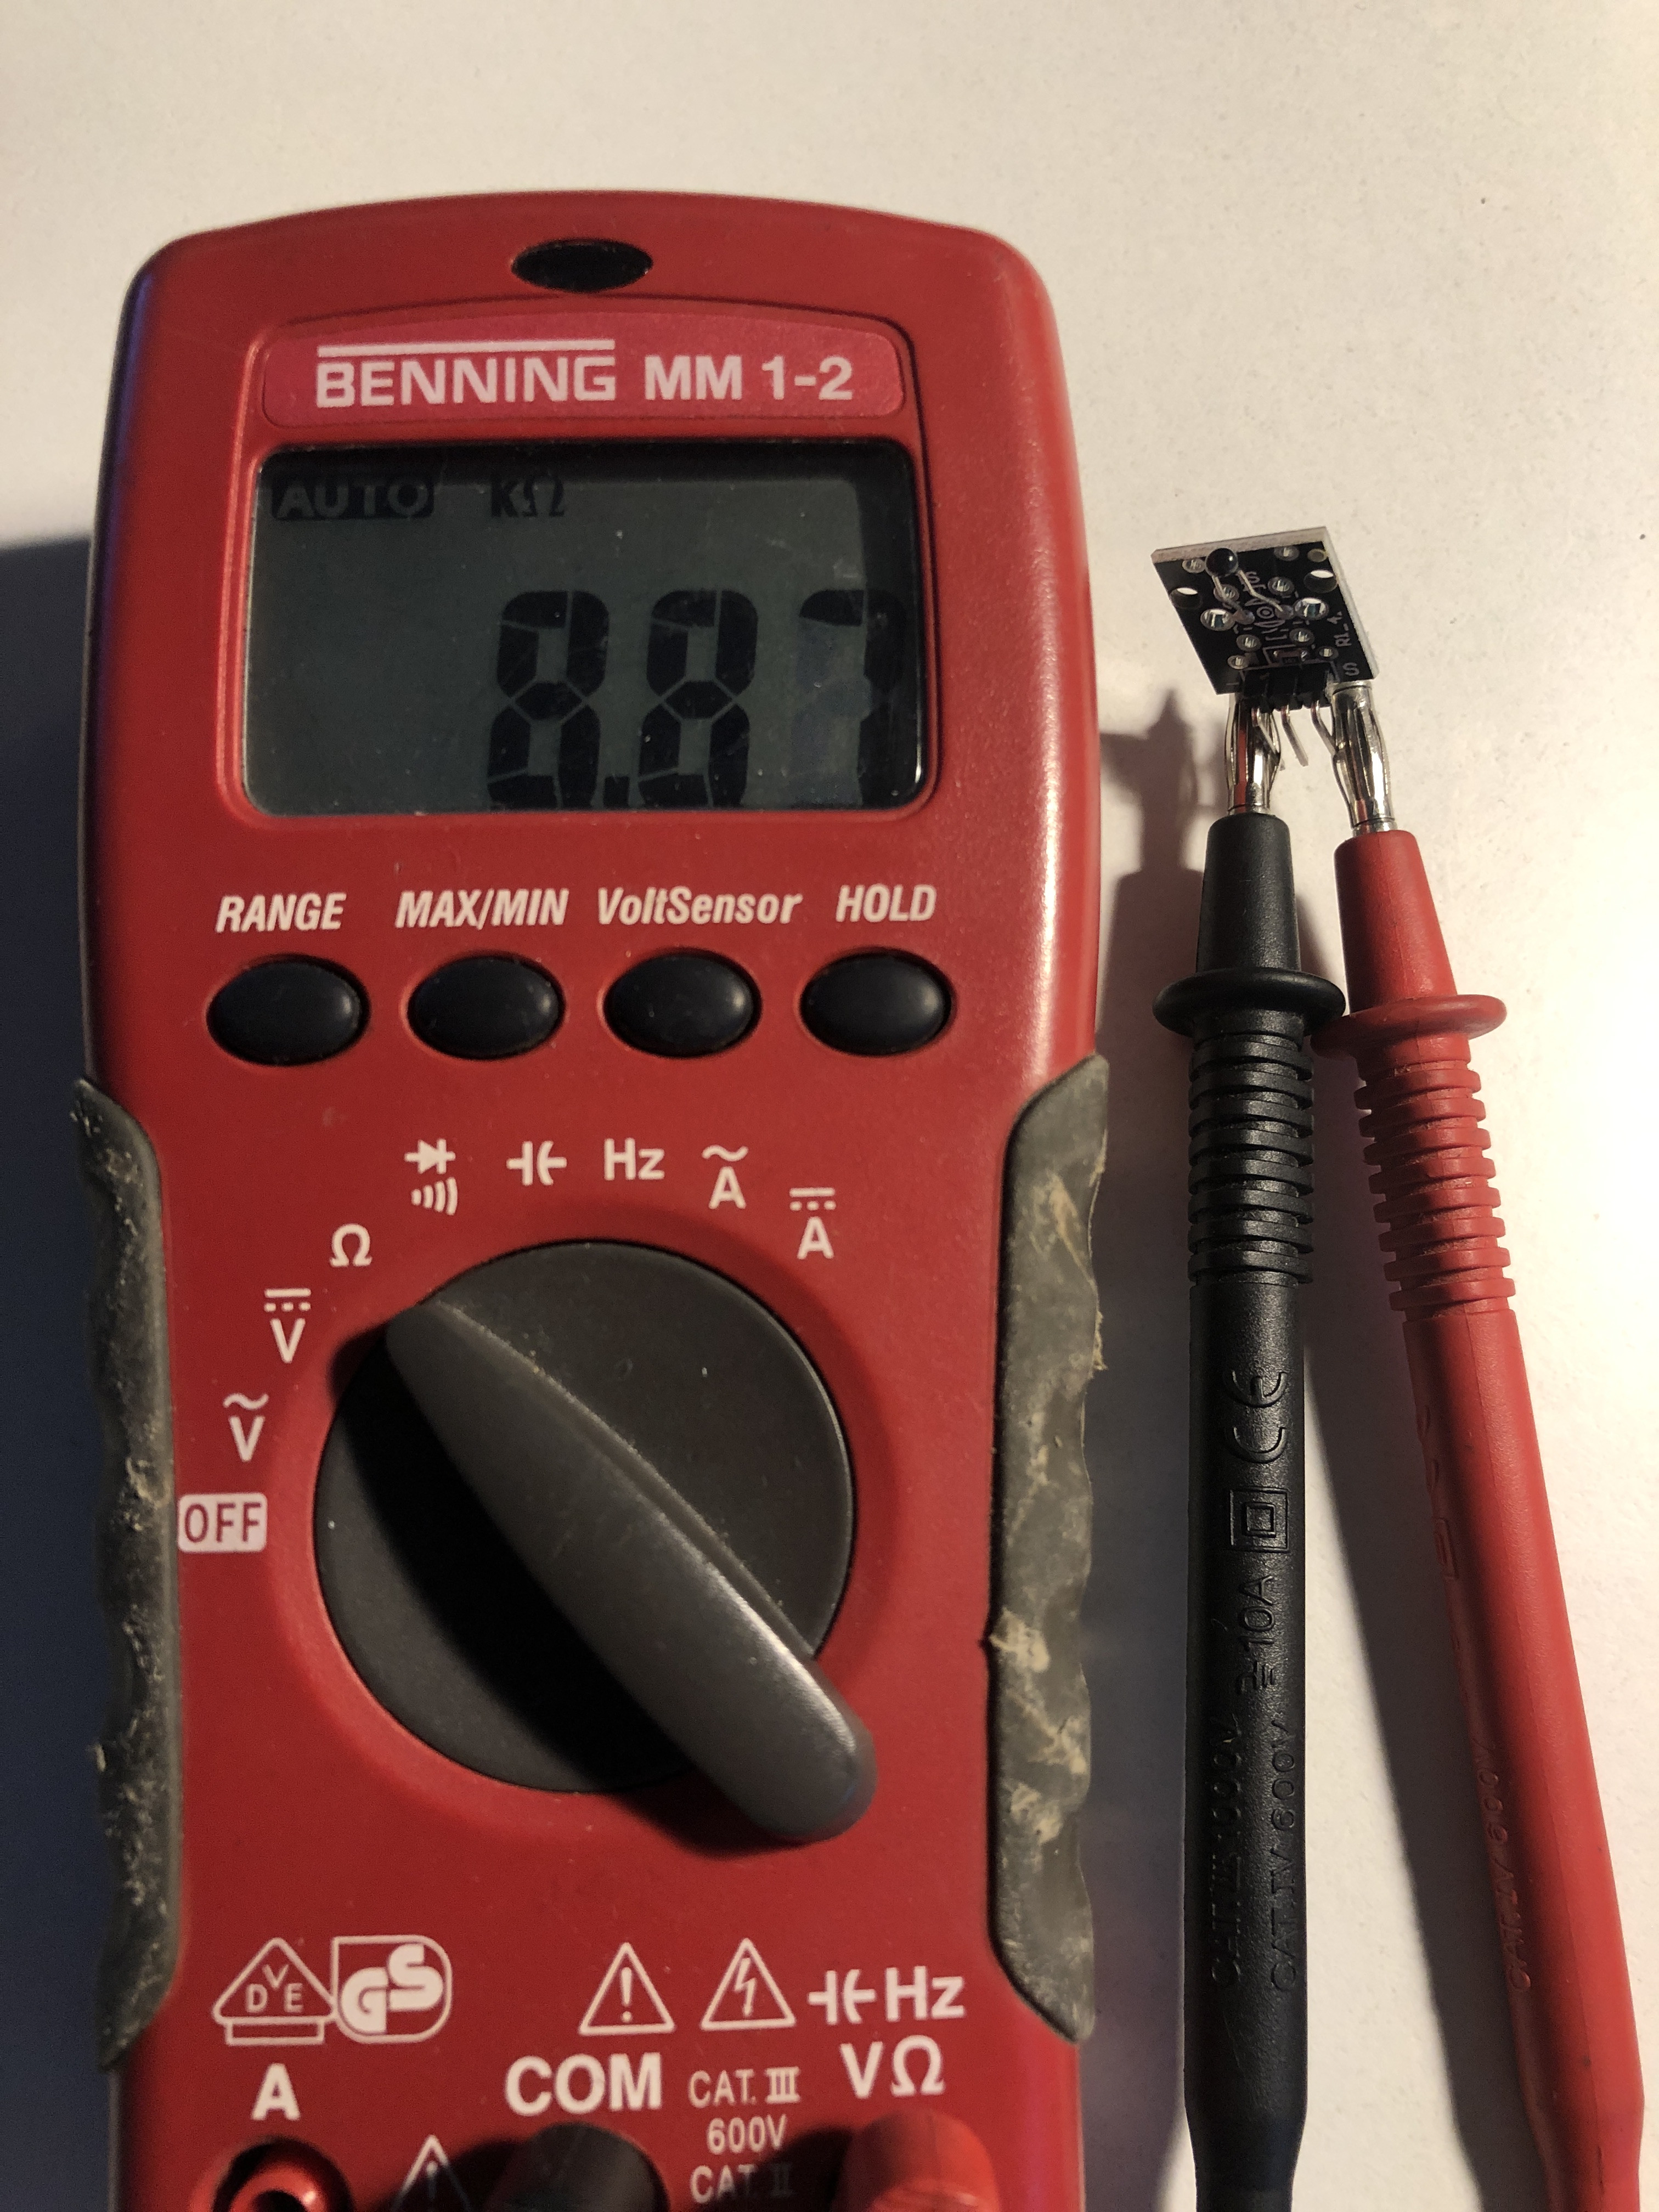
\includegraphics[width=.65\linewidth]{fig/KY-018/działanie_ukladu/1.jpg}
  \caption{Fotorezystor z pełnym dostępem do światła - 7.82k $\Omega$}
  \label{fig:sub1}
\end{subfigure}%
\begin{subfigure}{.5\textwidth}
  \centering
  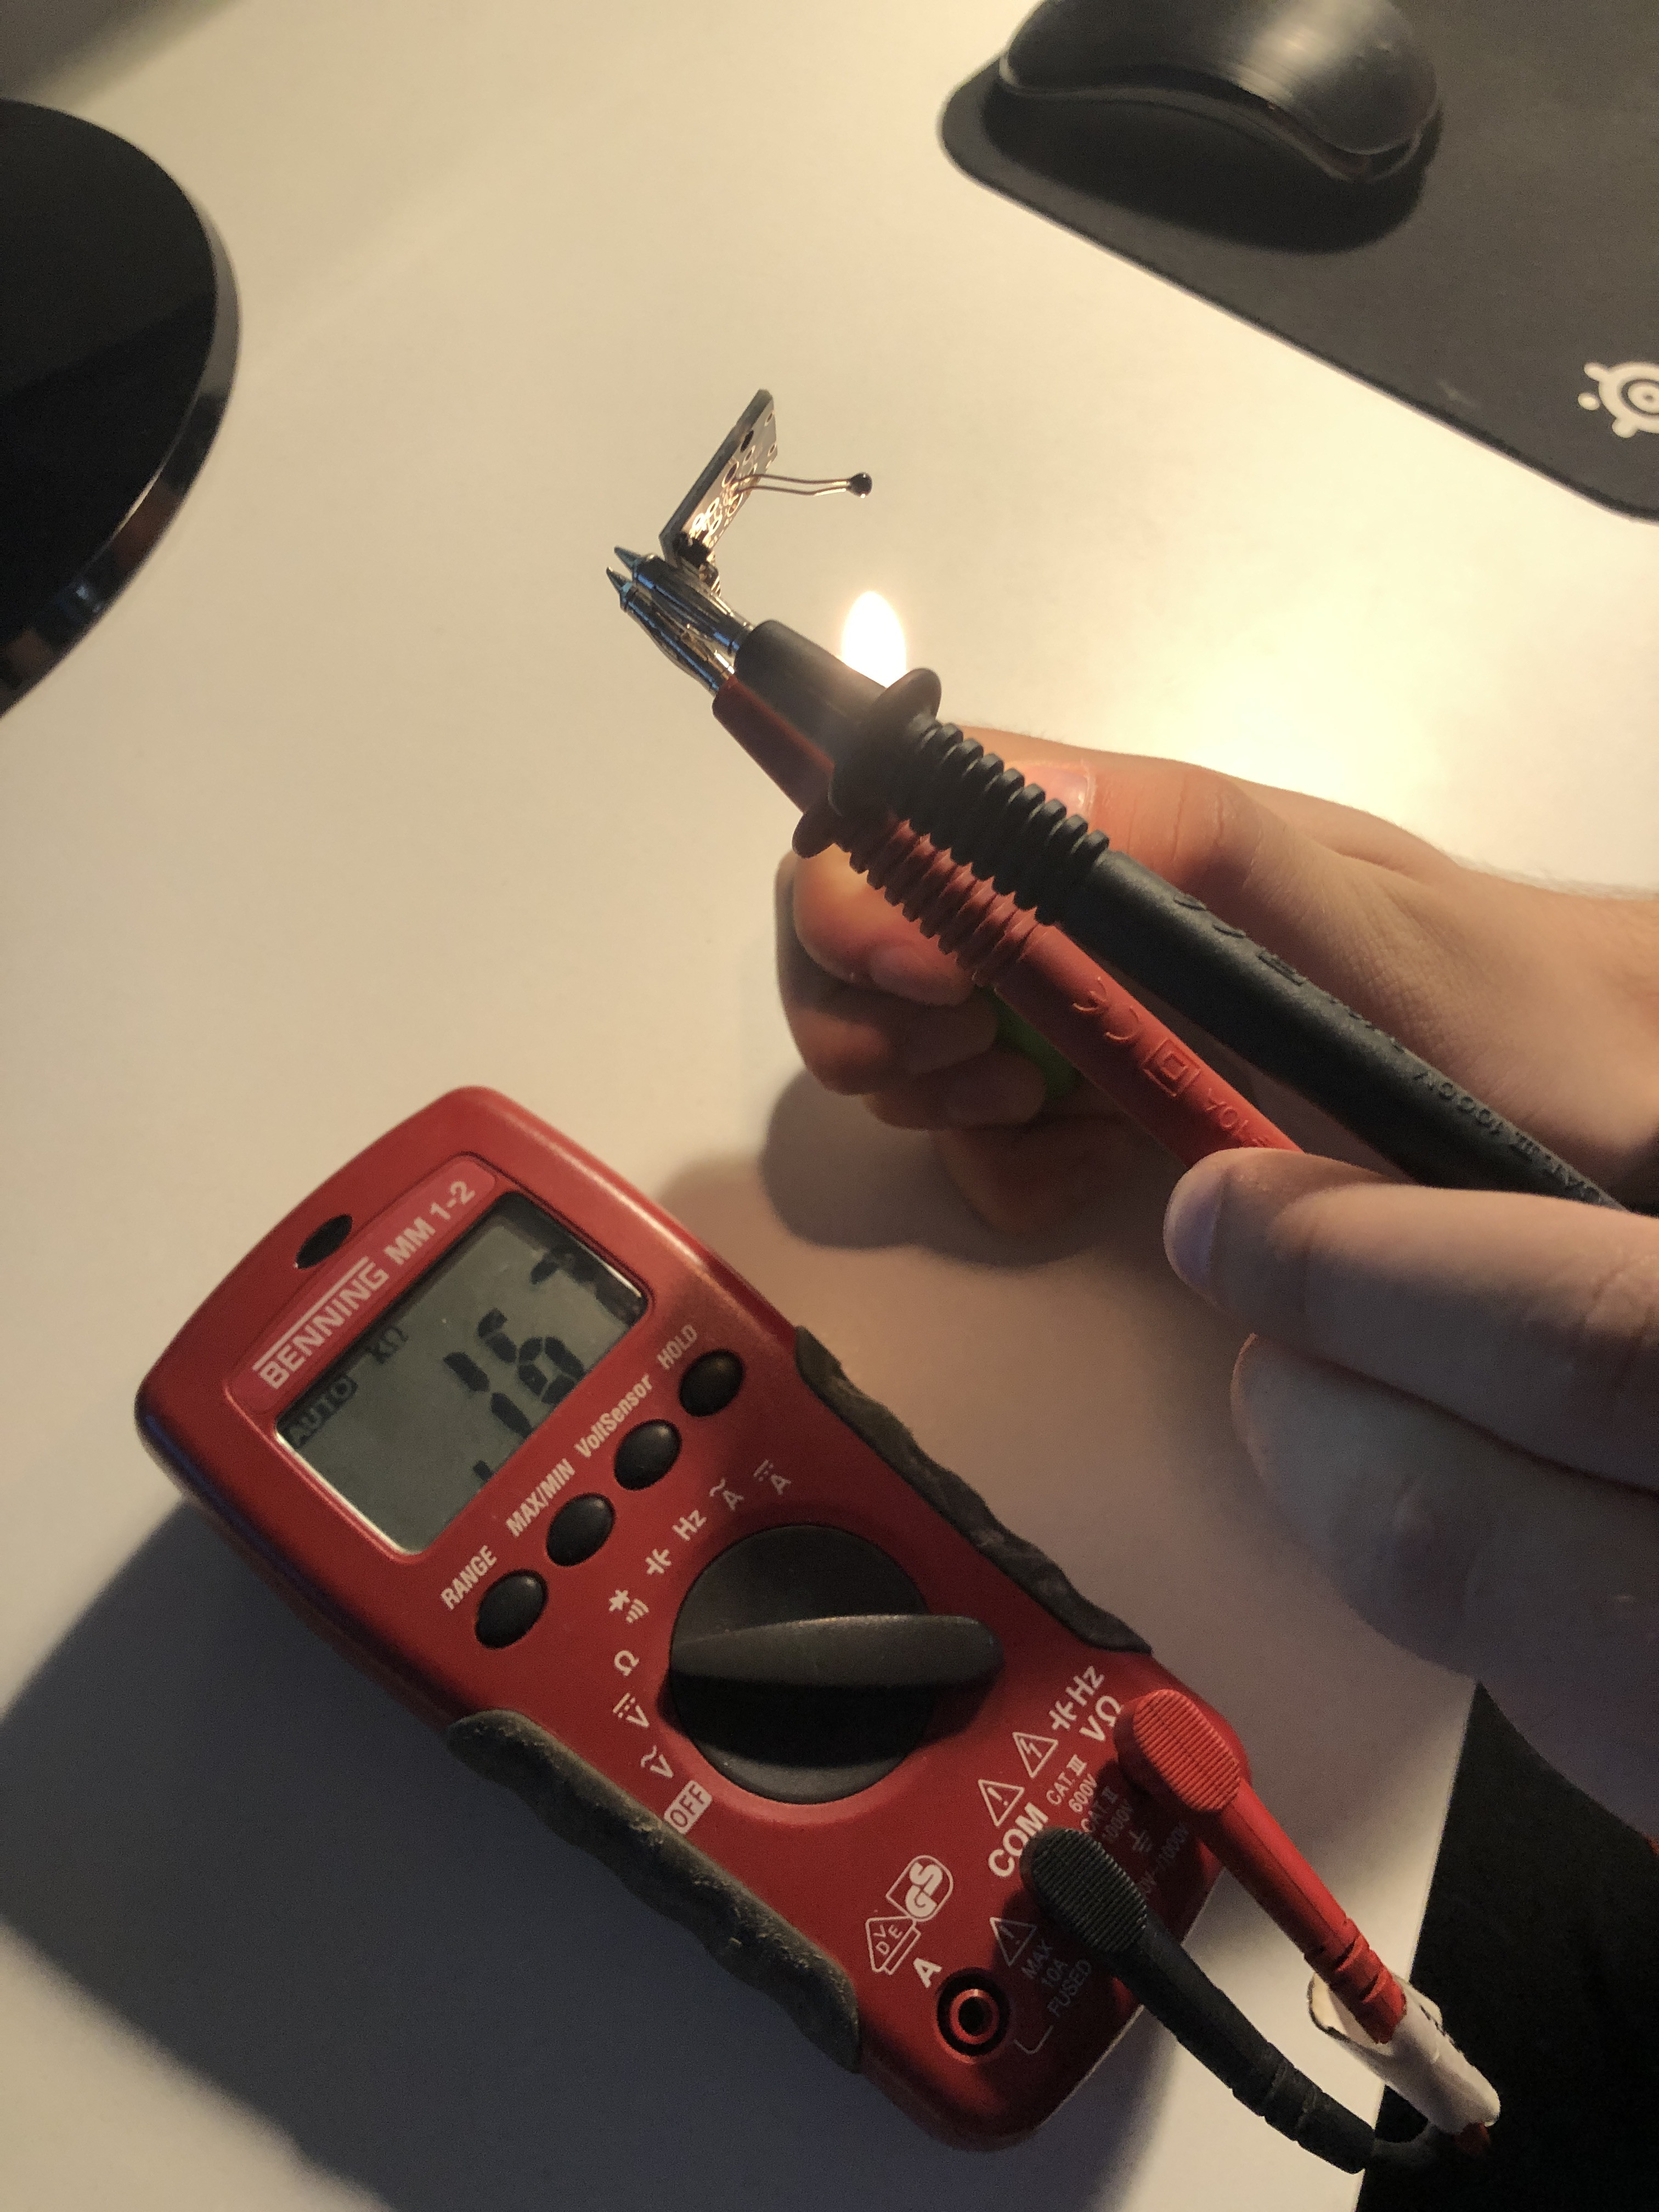
\includegraphics[width=0.65\linewidth]{fig/KY-018/działanie_ukladu/2.jpg}
  \caption{Fotorezystor zakryty w około 1/3 - 8.49k $\Omega$}
  \label{fig:sub2}
\end{subfigure}
\label{fig:test}
\begin{subfigure}{.5\textwidth}
  \centering
  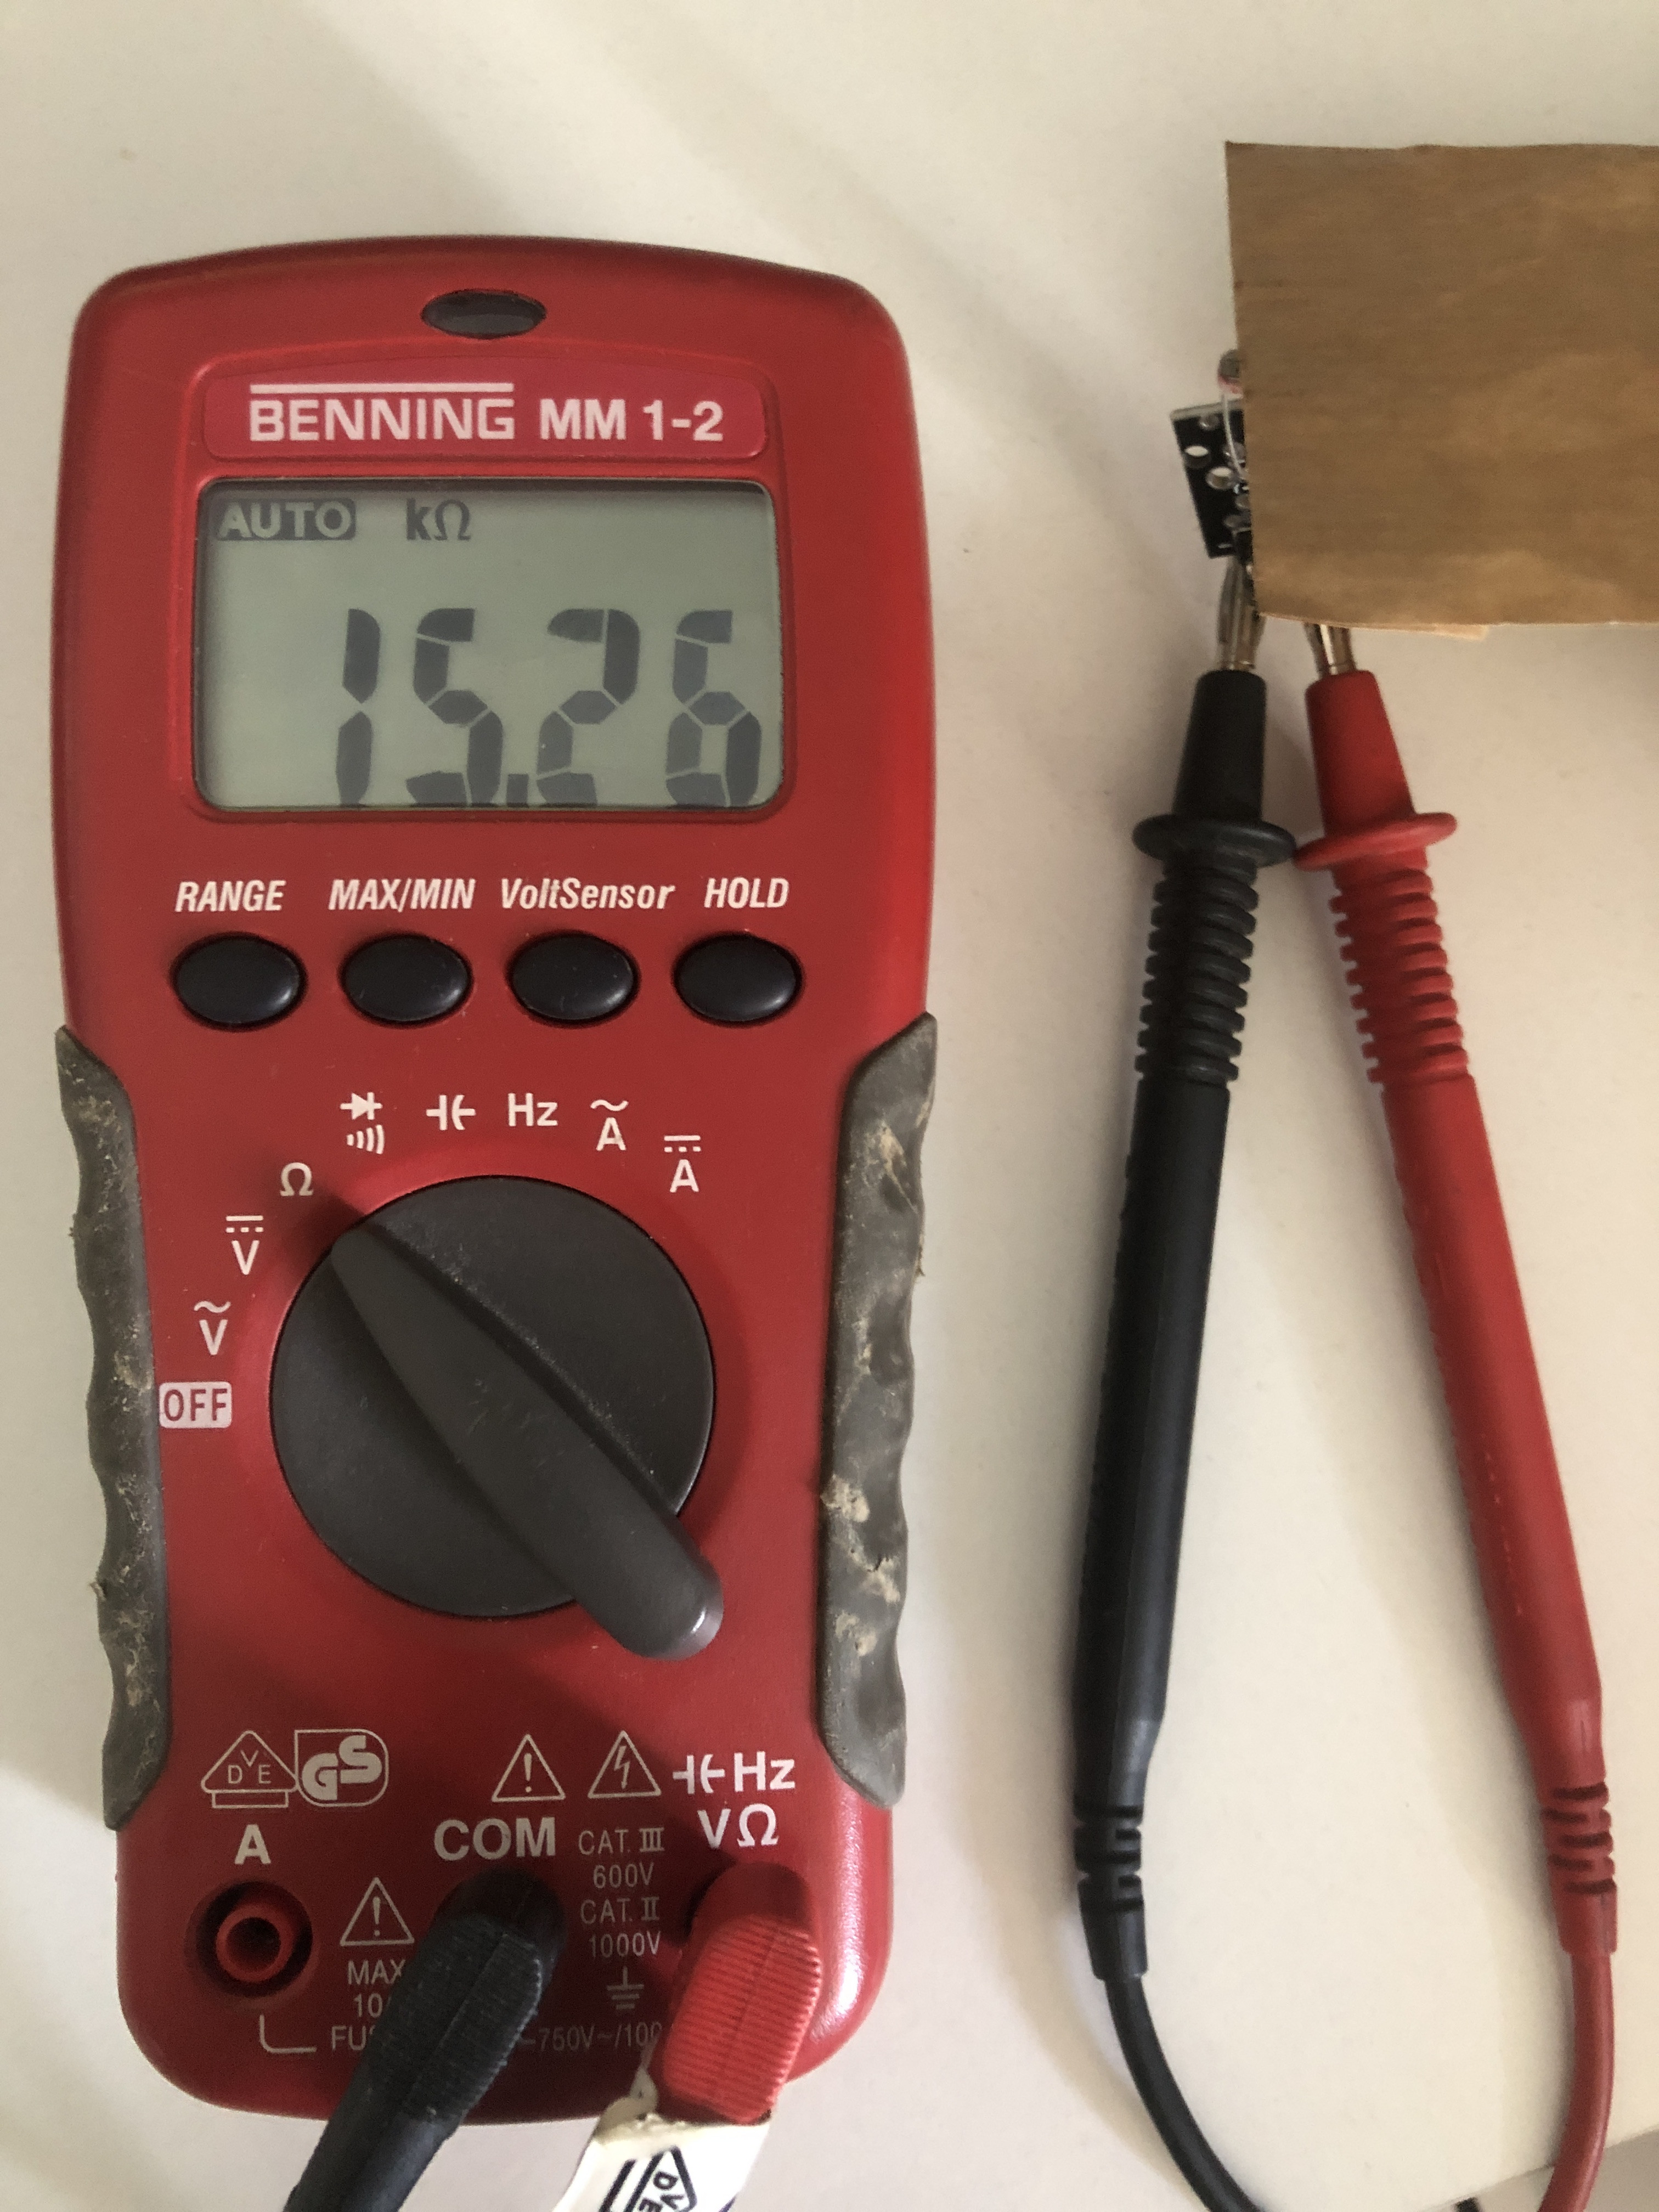
\includegraphics[width=.65\linewidth]{fig/KY-018/działanie_ukladu/3.jpg}
  \caption{Fortorezystor zakryty do połowy - 15.26k $\Omega$}
  \label{fig:sub3}
\end{subfigure}%
\begin{subfigure}{.5\textwidth}
  \centering
  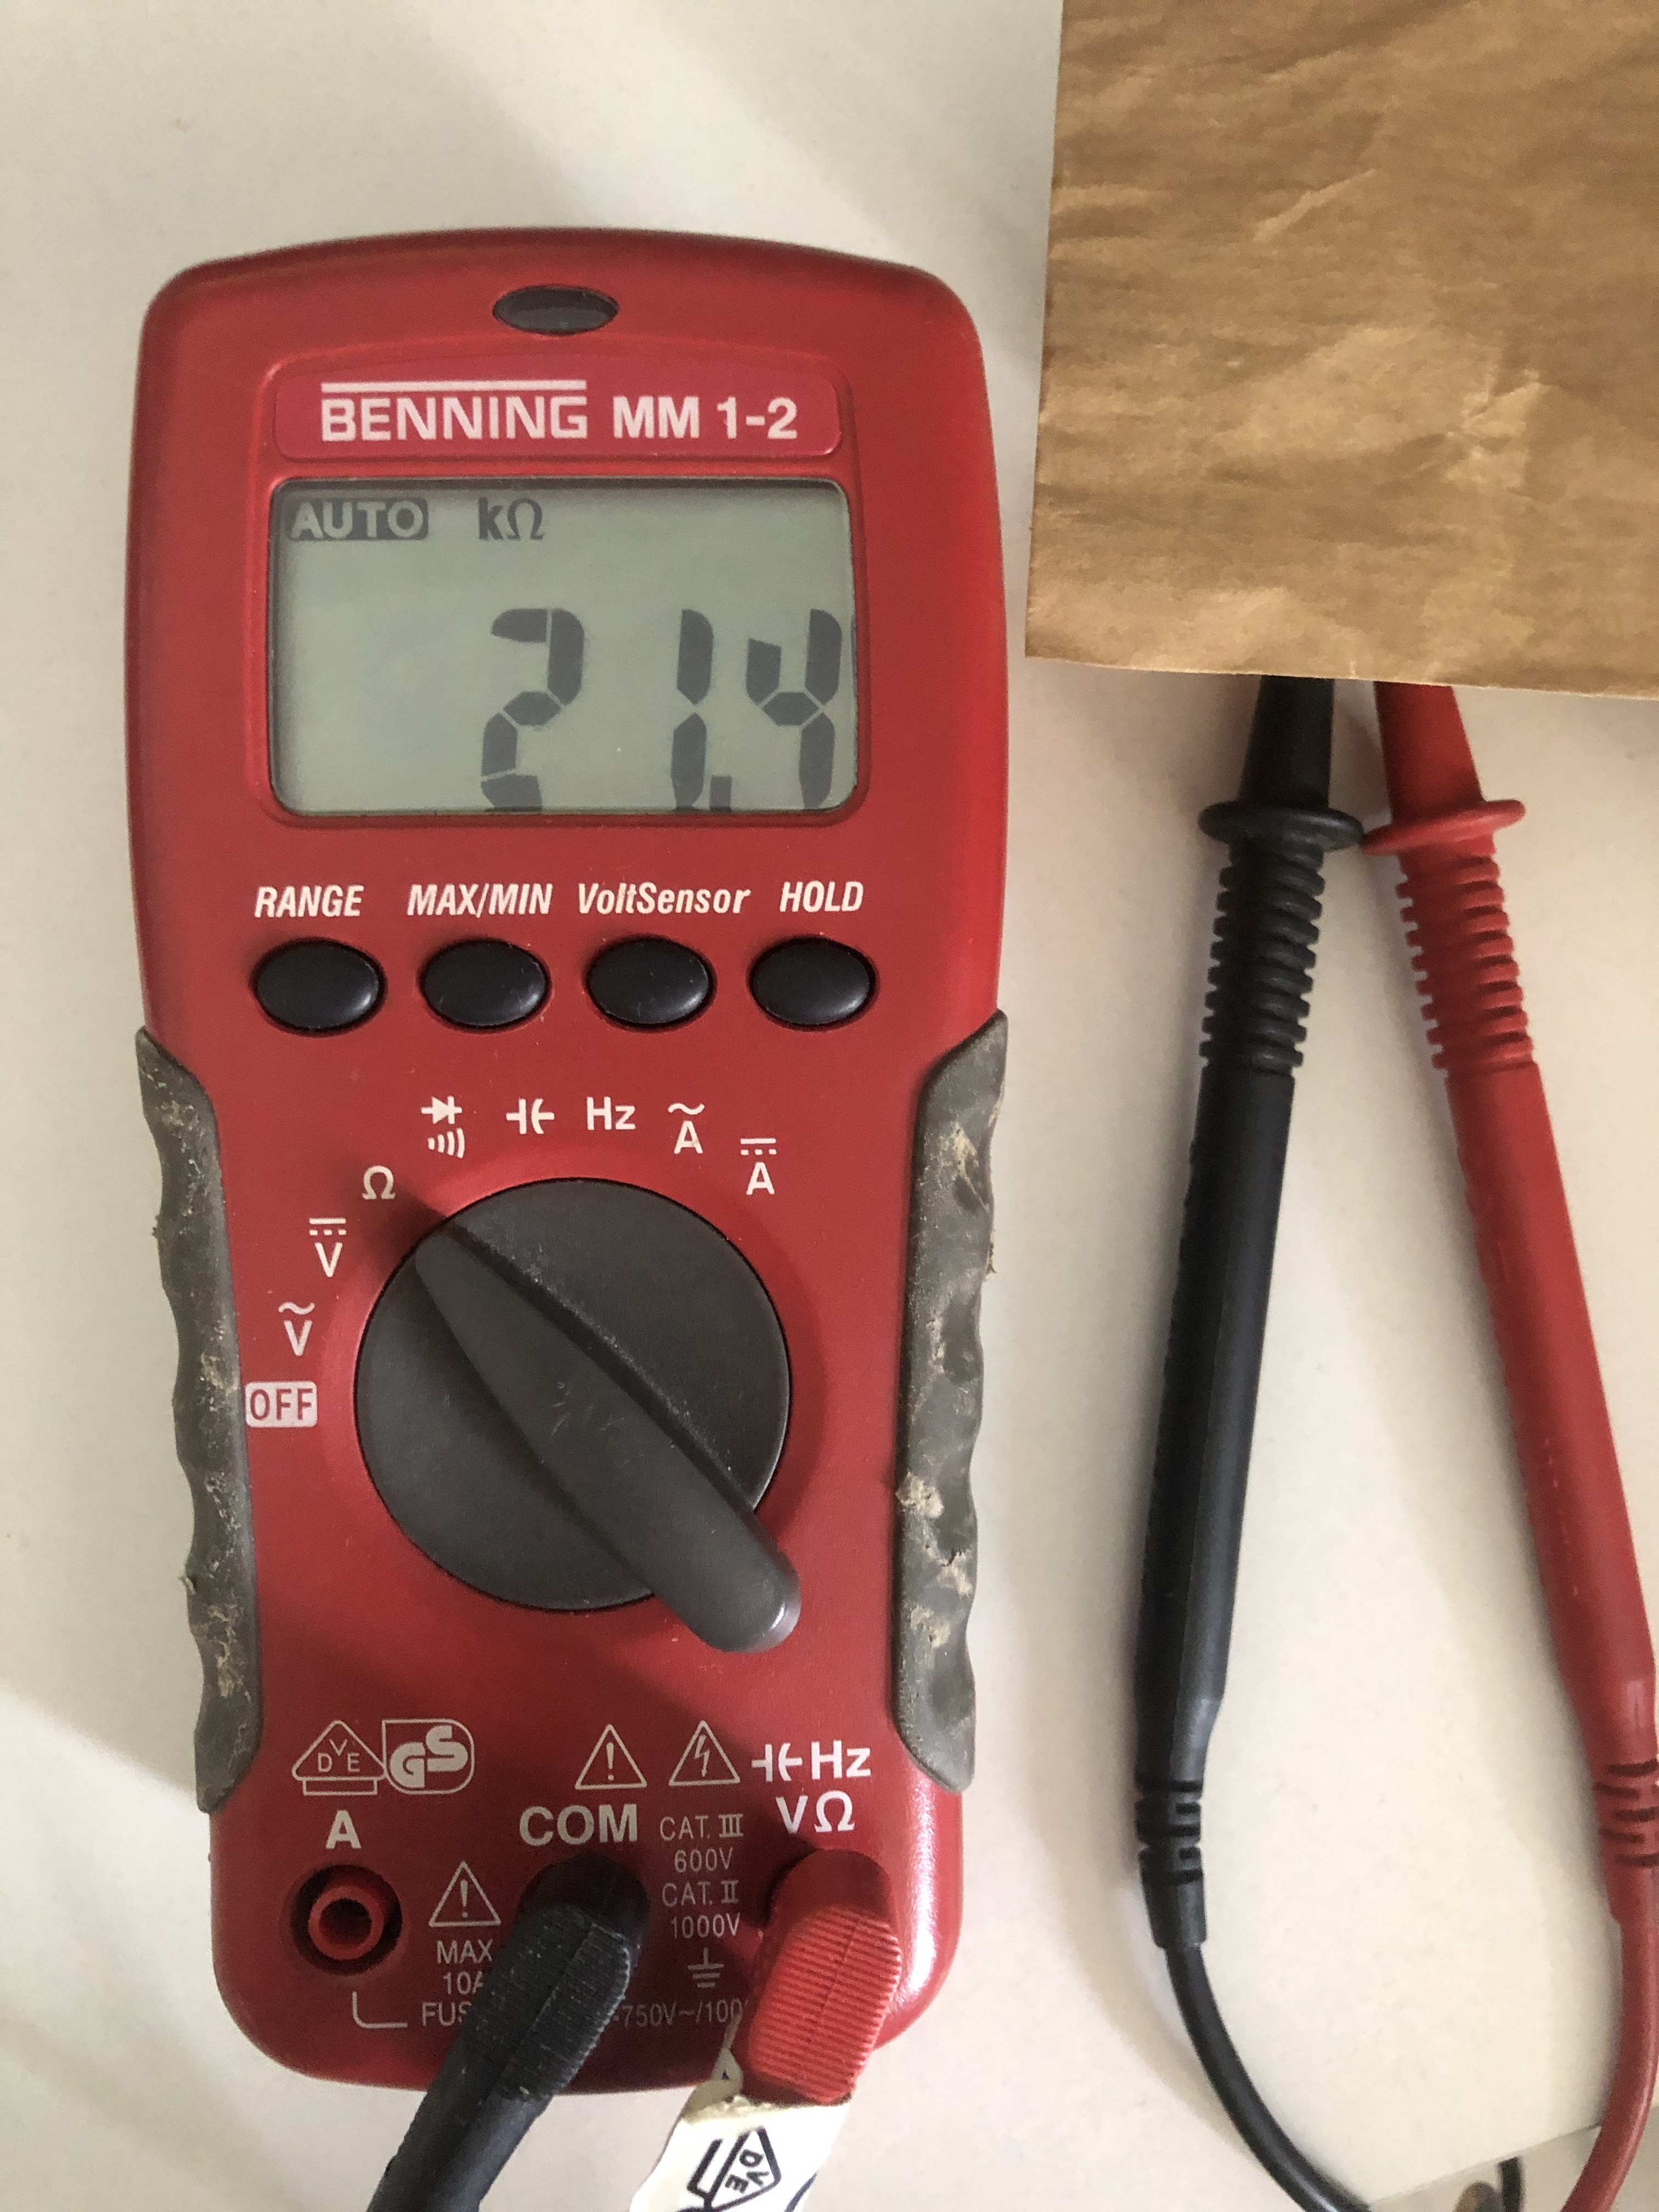
\includegraphics[width=0.65\linewidth]{fig/KY-018/działanie_ukladu/4.jpg}
  \caption{Całkowicie zakryty rezystor - 21.4k $\Omega$}
  \label{fig:sub4}
\end{subfigure}
\caption{Zmiana rezystancji modułu w zależności od dostępu do światła}
\label{fig:test}
\end{figure}
\newpage
Natężenie prądu fotorezystora określa wzór:
$$I=b\cdot U+d\cdot U\cdot \Phi^{\beta} $$
gdzie
\begin{itemize}
    \item $U$ - napięcie polaryzujące
    \item $\Phi$ - strumień świetlny
    \item $b, d, \beta$ - stałe zależne od materiału półprzewodnikowego i rodzaju domieszkowania
\end{itemize}
\vspace{0.5cm}
\begin{figure}[h!]
    \centering
    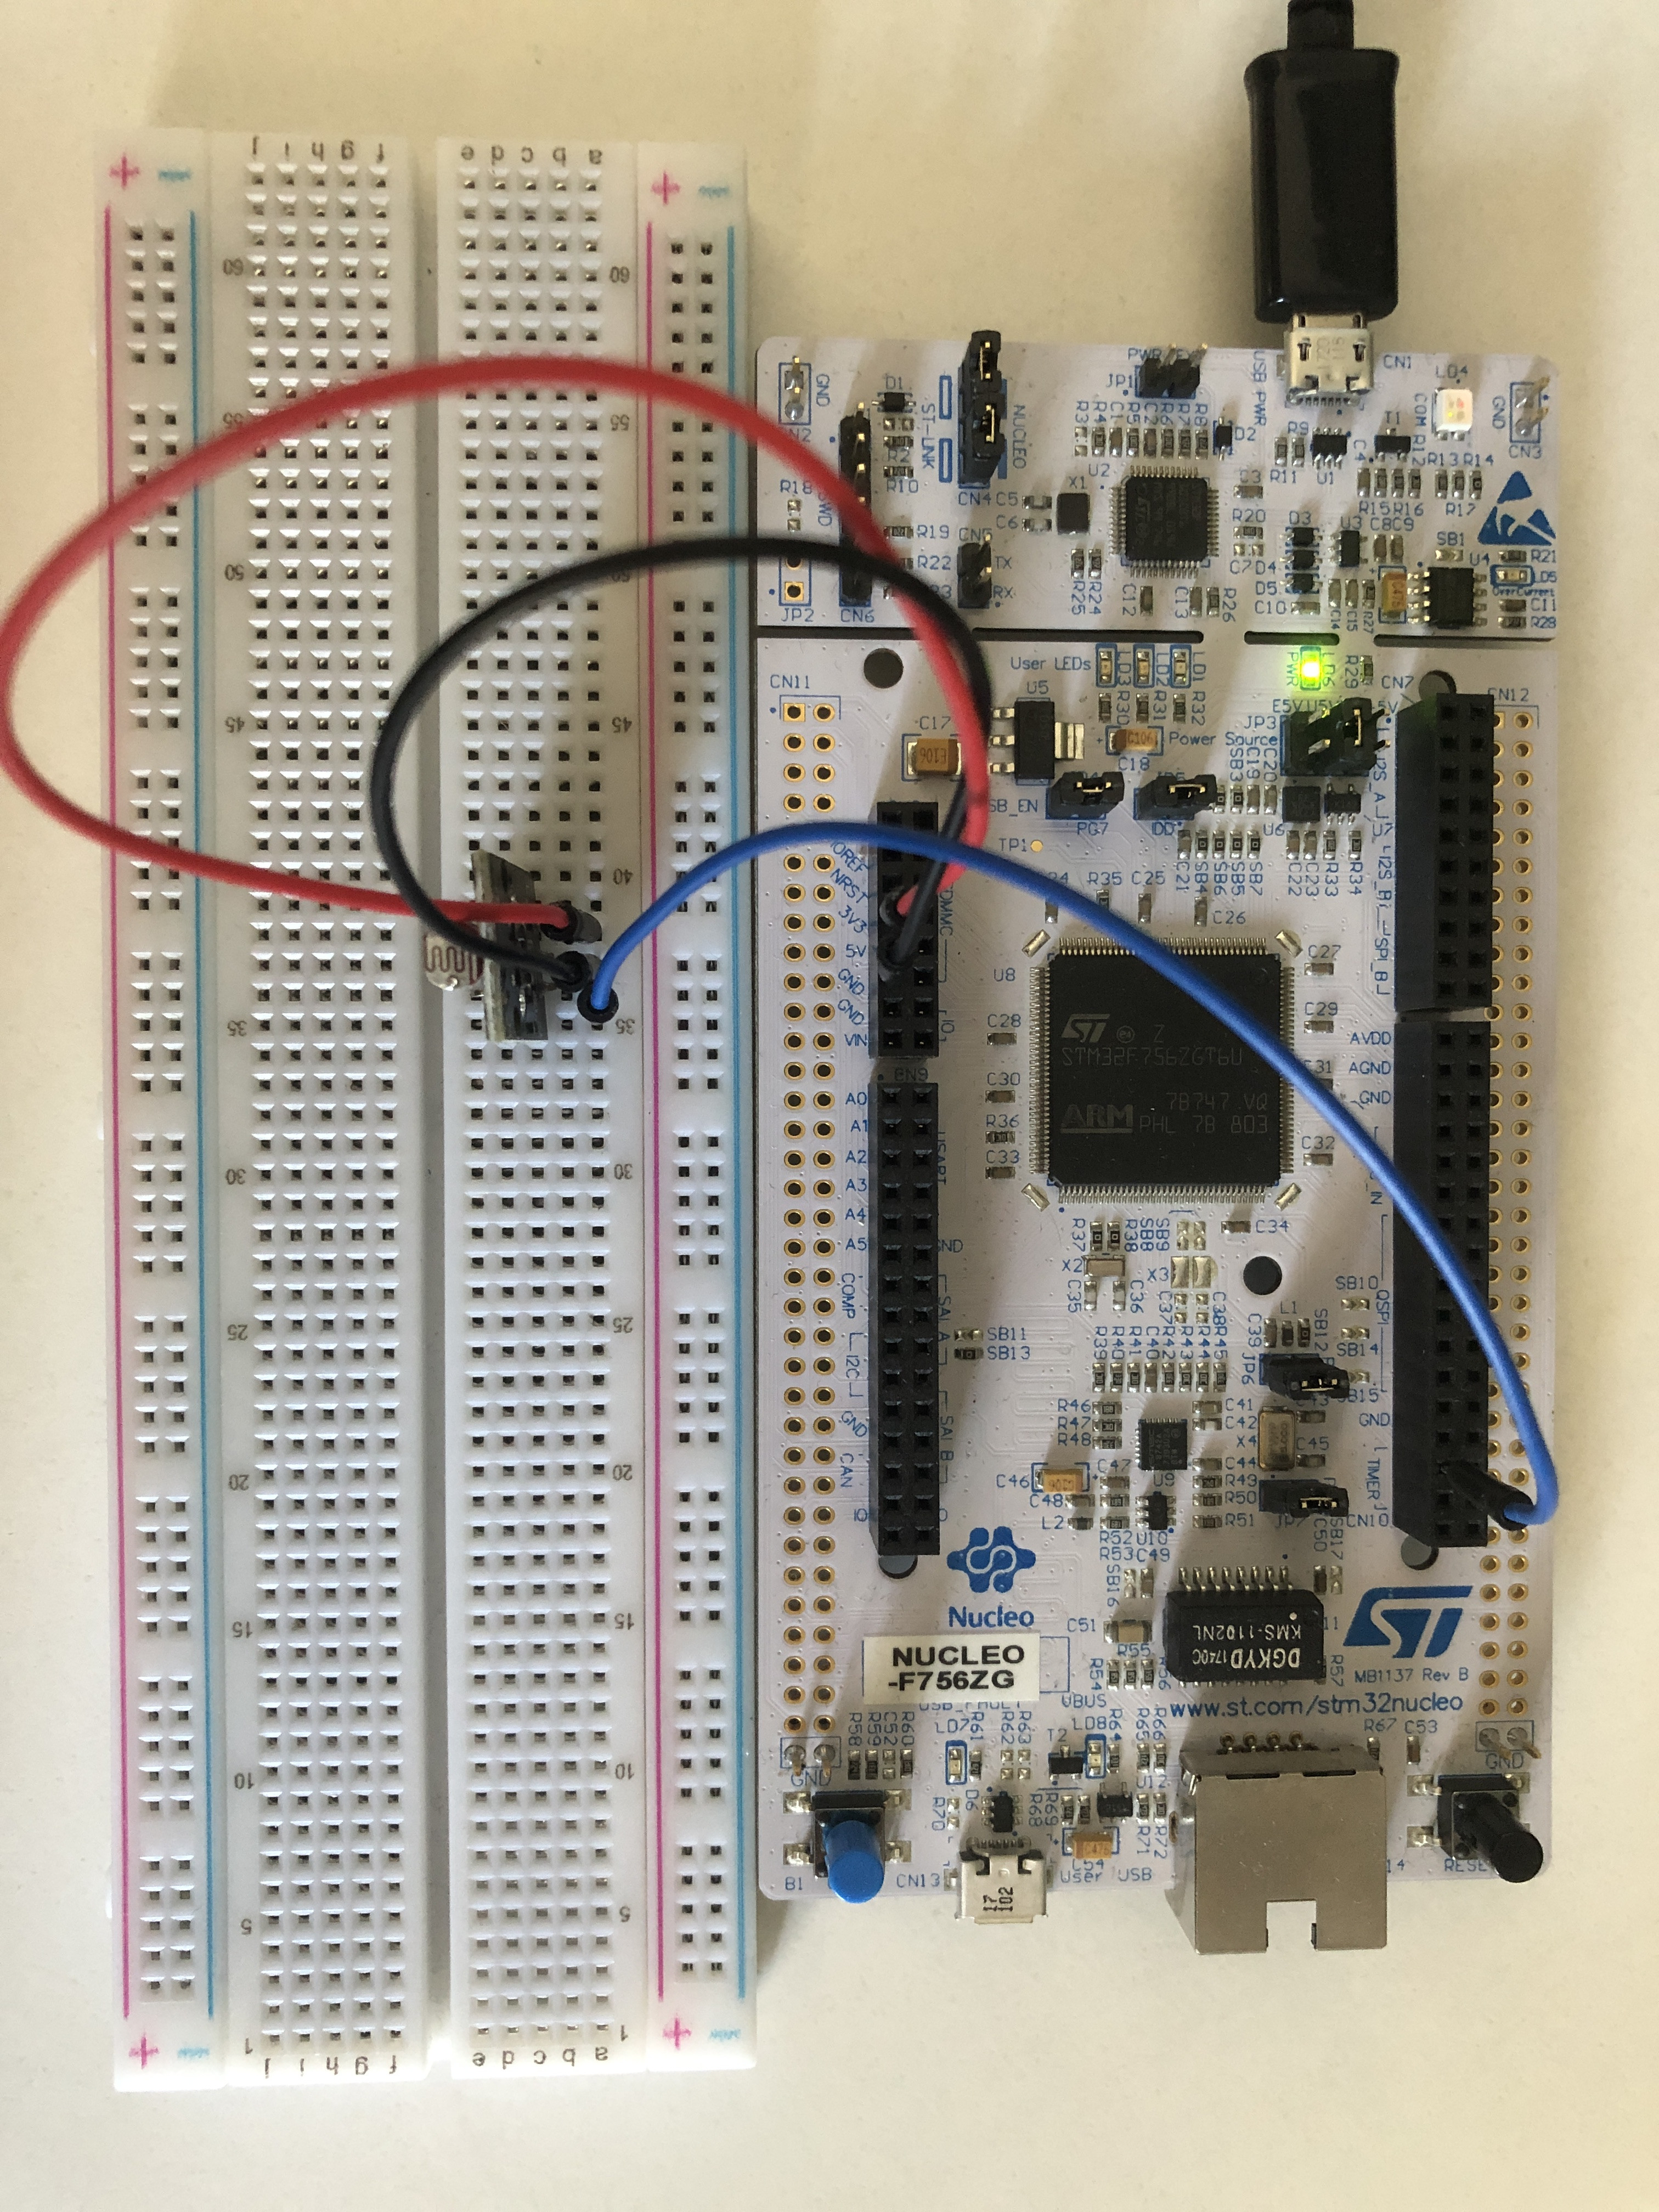
\includegraphics[width=0.45\textwidth,angle=90,origin=c]{fig/KY-018/działanie_ukladu/uklad.jpg}
    \caption{Przykład prostego podłączenia modułu z mikroprocesorem}
    \label{fig:my_label}
\end{figure}

\begin{figure}[h!]
\centering
\begin{subfigure}{.5\textwidth}
  \centering
  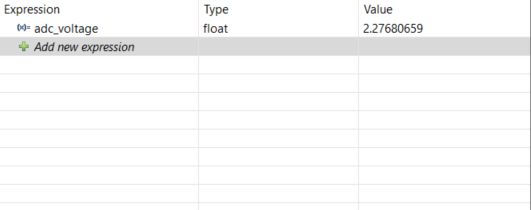
\includegraphics[width=1\linewidth]{fig/KY-018/działanie_ukladu/odkryte.png}
  \caption{Napięcie przy pełnym dostępie czujnika do światła}
  \label{fig:sub1}
\end{subfigure}%
\begin{subfigure}{.5\textwidth}
  \centering
  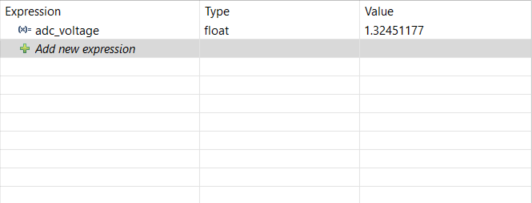
\includegraphics[width=1\linewidth]{fig/KY-018/działanie_ukladu/zakryte.png}
  \caption{Napięcie przy kompletnym zasłonięciu czujnika}
  \label{fig:sub2}
\end{subfigure}
\caption{Wartości napięcia w zależności od dostępu do światła}
\label{fig:test}
\end{figure}
\newpage

\begin{figure}[h!]
    \centering
    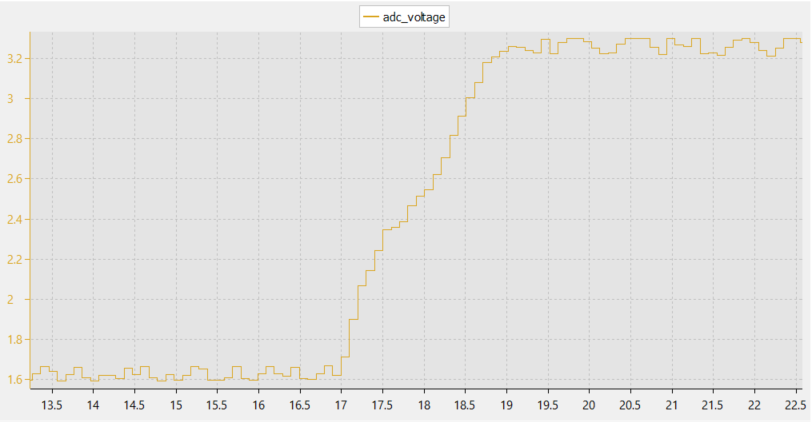
\includegraphics[width=1\linewidth]{fig/KY-018/działanie_ukladu/swv.png}
    \caption{Odczyt zmiany napięcia w zależności od dostępu światła do czujnika}
    \label{fig:my_label}
\end{figure}

Na Rys.6 można zaobserwować zmianę napięcia w czasie, które spodowowane jest ograniczeniem dostępu światła padającego na powierzchnię światłoczułą fotorezystora wbudowanego w moduł. Wartość najwyższa występuje w przypadku, gdy fotorezystor jest kompletnie odkryty - rezystancja jest najmniejsza, natomiast najniższe napięcie osiągane jest przy pełnym zakryciu czujnika.
\newline

Kod programujący czujnik, wykorzystany do opracowania instrukcji, znajduje się w materiałach dodatkowych zawartych pod koniec rozdziału.
\newline
Film prezentujący działanie układu znajduje się w suplemencie wideo.
\printbibliography[heading=bibintoc]

\end{document}